\documentclass[aspectratio=169]{beamer}
\usepackage[utf8]{inputenc}
\usepackage[brazil]{babel}
\usepackage{multimedia,amsmath,graphicx,color,multicol,fancyhdr,amssymb,amsfonts,amsthm,setspace}
\usepackage{ragged2e}
\usetheme{Berlin}
\usecolortheme{dolphin}
\usepackage{setspace}
\usepackage{xcolor}
\usepackage{graphicx}
\usepackage{textcomp}

% Informações que serão inseridas no slide da capa:
\title[CETi Gilberto Mestrinho]{Aulão de Revisão - Matemática - PSC 2}
%\author[Prof. Joao Victor]{Prof. Joao Victor}
%\institute[IFAM]{Instituto Federal do Amazonas}
\date{6 de junho de 2025} 
%\logo{
\includegraphics[scale=0.05]{logo-utfpr.png}} 

\newif\ifusarcorvermelha
%\usarcorvermelhatrue % Ativa o texto vermelho (comente para desativar)

% --- Comando \vermelho ---
\newcommand{\vermelho}[1]{%
    \ifusarcorvermelha
        {\color{red}#1}% % Texto vermelho se \ifusarcorvermelha = true
    \else
        #1% % Texto normal se \ifusarcorvermelha = false
    \fi
}

\begin{document}
\justifying
\onehalfspacing

\begin{frame}
    \begin{titlepage}
    \centering
    \vspace*{1cm} % Ajuste o espaçamento vertical conforme necessário
    
    % Logos alinhadas horizontalmente
    \noindent%
    \hspace*{0.3\paperwidth}%
    
\includegraphics[height=2cm,keepaspectratio]{logo_ufam.jpg}%
    \hfill%
    
\includegraphics[height=2cm,keepaspectratio]{logo_ceti.png}%
    \hspace*{0.3\paperwidth}%
    
    \vspace{0.1cm} % Espaço entre as logos e o título

    \vspace{1cm}
    
    \vfill % Preenche o espaço vertical restante
    \end{titlepage}
\end{frame}

\begin{frame}{Conteúdo Programático - PSC 2}

    \begin{center}
        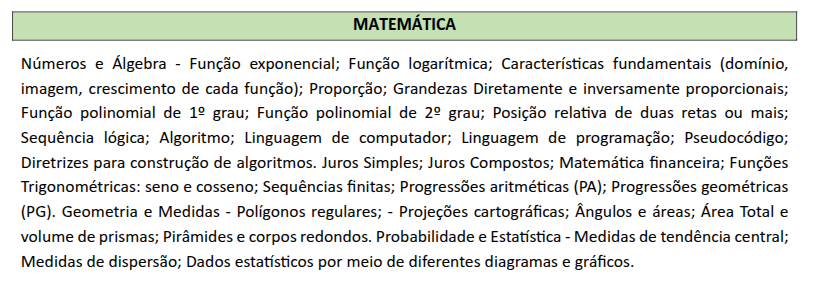
\includegraphics[scale=0.5]{psc2.png}
    \end{center}
    
\end{frame}

\section{Geometria Espacial}

    \begin{frame}{1. PSC 2 - 2024 (Questão 47)}
        Estudos demográficos revelam que a população de certo país, no ano zero, é $f_{0}$ e, decorridos $t$ anos, a população poderá ser estimada pela função: $f(t)=f_{0} \times  e^{0,05 . t}$. Considerando $\ln{3}=1,10$, podemos afirmar que a população desse país deverá triplicar quando decorrerem, aproximadamente,

            \begin{enumerate}[a]
                \item 10 anos.
                \item 16 anos.
                \item 18 anos.
                \item 20 anos.
                \item \vermelho{22 anos.} %
            \end{enumerate}
            
    \end{frame}


    \begin{frame}{2. PSC 2 - 2024 (Questão 48)}
        Seja a função $f: \mathbb{R} \to \mathbb{R}$, definida por $f(x)=9^{x+1}$. O valor de $x$, de modo que $f(4-x)=3f(x)$, deve ser:
        
            \begin{enumerate}[a]
                \item {3}/{4}
                \item {5}/{4}
                \item \vermelho{{7}/{4}} %
                \item {5}/{6}
                \item {7}/{6}
            \end{enumerate}
            
    \end{frame}

    \begin{frame}{4. PSC 2 - 2024 (Questão 50)}
        Em uma aula de geometria, a professora de Matemática orientou os alunos para que construíssem uma pirâmide de base quadrada com 4,0 cm de lado e 12 cm de altura. O volume dessa pirâmide é igual a:

         \begin{enumerate}[a]
                    \item $36 \ cm^{3}$
                    \item $48 \ cm^{3}$
                    \item $52 \ cm^{3}$
                    \item \vermelho{$64 \ cm^{3}$} %
                    \item $72 \ cm^{3}$
                \end{enumerate}        
    \end{frame}

    \begin{frame}{5. PSC 2 - 2024 (Questão 51)}
        Uma avenida possui 4055 m de extensão e vai receber em seu canteiro central o plantio de árvores de pequeno porte. A distância entre as mudas deve ser de 16 m, com a primeira árvore sendo plantada a 7 m do início da avenida. A quantidade de árvores que deverão ser plantadas será igual a:


         \begin{enumerate}[a]
                    \item $248$
                    \item \vermelho{$254$} %
                    \item $276$
                    \item $320$ 
                    \item $342$
                \end{enumerate}        
    \end{frame}

    \begin{frame}{6. PSC 2 - 2024 (Questão 52)}
       Para a existência da expressão: $\cos(x) = \dfrac{3x-2}{4}$. Os valores de x  devem estar compreendidos no intervalo:


         \begin{enumerate}[a]
                    \item \vermelho{$-{2}/{3} \leq x \leq 2$} %
                    \item $-1 \leq x \leq 1$
                    \item $-1 \leq x \leq 2$
                    \item $-2 \leq x \leq 3$
                    \item $-{7}/{3} \leq x \leq 4$
                \end{enumerate}        
    \end{frame}

    \begin{frame}{7. PSC 2 - 2024 (Questão 53)}
      Considere a progressão geométrica $(1, 4, 16, 64, … )$. A quantidade de termos que devem ser somados, para que o resultado da adição seja 87381, é igual a:


         \begin{enumerate}[a]
                    \item 8
                    \item \vermelho{9} %
                    \item 10
                    \item 13
                    \item 16
                \end{enumerate}        
    \end{frame}

    \begin{frame}{8. PSC 2 - 2024 (Questão 54)}
      Para a função real definida por: $f(x)=(k-3)x^{2}-5x-6$, é \textbf{CORRETO} afirmar que:

         \begin{enumerate}[a]
                    \item se $k=4$, então $f(-1)=1.$
                    \item o gráfico de $f(x)$ é uma parábola para todo $k \in \mathbb{R}$.
                    \item \vermelho{se $k=1$, então $f(x)$ é negativa para todo $x \in \mathbb{R}$} %
                    \item se $k = 4$, então $f(6)=2$
                    \item se $k <3$, então o gráfico de $f(x)$ é uma parábola com a concavidade voltada para cima.
                \end{enumerate}        
    \end{frame}

    \begin{frame}{9. PSC 2 - 2023 (Questão 47)}
      Sejam $\alpha$ e $\beta$, respectivamente, os determinantes das matrizes não singulares:

      \begin{center}
          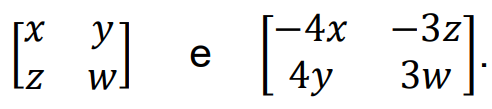
\includegraphics[scale=0.5]{QuestaoPSC2023Q47.png}
      \end{center} Logo, a razão ${\beta}/{\alpha}$?
      
         \begin{enumerate}[a]
                    \item $-14$
                    \item \vermelho{$-12$} %
                    \item $10$
                    \item $12$
                    \item $14$
                \end{enumerate}        
    \end{frame}

     \begin{frame}{10. PSC 2 - 2023 (Questão 48)}
        Considerando que o conjunto A possui 5 elementos e o conjunto B, 8 elementos, podemos afirmar que a quantidade de funções injetoras $f:A \to B$ que podemos formar é:

         \begin{enumerate}[a]
                    \item 7200.
                    \item 8740.
                    \item \vermelho{6720.} %
                    \item 25900.
                    \item 32768.
                \end{enumerate}        
    \end{frame}

     \begin{frame}{11. PSC 2 - 2023 (Questão 49)}
        Uma piscina tem 10 m de comprimento, 8 m de largura e 1,8 m de profundidade. O volume, em litros, dessa piscina é:

         \begin{enumerate}[a]
                    \item 110000.
                    \item 115000.
                    \item 115000.
                    \item 132000.
                    \item \vermelho{144000.} %
                \end{enumerate}        
    \end{frame}

    \begin{frame}{12. PSC 2 - 2023 (Questão 50)}
       Uma pirâmide regular, de base quadrada, possui área da base igual a $50 \ dm^{2}$. Sabendo que o apótema da pirâmide mede $6 \ dm$ , podemos afirmar que a altura dessa pirâmide mede:


         \begin{enumerate}[a]
                    \item \vermelho{$\sqrt{23,5}$} dm %
                    \item $\sqrt{32,5}$ dm
                    \item $\sqrt{42,5}$ dm
                    \item $\sqrt{53,5}$ dm
                    \item $\sqrt{64,5}$ dm
                \end{enumerate}        
    \end{frame}

    \begin{frame}{13. PSC 2 (Questão 52)}
       Assinale a alternativa \textbf{CORRETA}:


         \begin{enumerate}[a]
                    \item Dois planos que possuem três pontos em comum são coincidentes.
                    \item Se dois planos $\alpha$ e $\beta$ são perpendiculares ao plano $\gamma$, então os planos $\alpha$ e $\beta$ são paralelos.
                    \item Existem dois planos distintos, passando ambos por um mesmo ponto e perpendiculares a uma reta.
                    \item \vermelho{Duas retas perpendiculares a um plano são paralelas.} %
                    \item Toda reta paralela a um plano é perpendicular a infinitas retas desse plano.

                \end{enumerate}        
    \end{frame}

    \begin{frame}{14. PSC 2 - 2023 (Questão 53)}
      Um cilindro reto possui área total igual a $32\pi \ cm^{2}$. Sabendo que o raio da base é ${1}/{3}$ da medida da altura desse cilindro, então a área lateral desse cilindro mede:
       
         \begin{enumerate}[a]
                    \item $12\pi \ cm^{2}$
                    \item $18\pi \ cm^{2}$
                    \item $20\pi \ cm^{2}$
                    \item \vermelho{$24\pi \ cm^{2}$} %
                    \item $28\pi \ cm^{2}$

                \end{enumerate}        
    \end{frame}

    \begin{frame}{15. PSC 2 - 2023 (Questão 54)}
        A quantidade de anagramas distintos de $ANO2013$ que é possível formar, de modo que comecem por uma letra e terminem em um número é:
       
         \begin{enumerate}[a]
            \item 680.
            \item 720.
            \item \vermelho{1440.}
            \item 840.
            \item 925.

        \end{enumerate}        
    \end{frame}

    \begin{frame}{16. PSC 2 - 2022 (Questão 47)}
        Dois recipientes, um cilíndrico e um cônico, têm a mesma altura e bases com raios iguais. Se a capacidade do recipiente cônico é de $205 mL$, então a capacidade do recipiente cilíndrico é de:

        \begin{enumerate}[a]
            \item $205\ ml$
            \item $410\ ml$
            \item $505\ ml$
            \item \vermelho{$615\ ml$} %
            \item $750\ ml$

        \end{enumerate}        
    \end{frame}

    \begin{frame}{16+1. PSC 2 - 2022 (Questão 50)}
        Sejam as matrizes:

        \begin{center}
            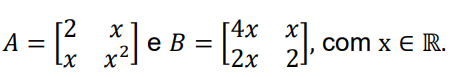
\includegraphics[scale=0.5]{questãoPSC2022Q50.png}
        \end{center} Os valores de $x$ que tornam verdadeira a igualdade $det\  A = 4 \times det\ B$ são $x=0$ ou:

        \begin{enumerate}[a]
            \item $x={16}/{3}$
            \item $x={26}/{9}$
            \item \vermelho{$x={32}/{9}$} %
            \item $x={32}/{3}$
            \item $x={3}/{16}$

        \end{enumerate}        
    \end{frame}

    \section{Adicionais}

        \begin{frame}{ PSC  - 2024 (Questão 53)}
        Considere o conjunto de dados apresentados pela seguinte distribuição de frequência:

        \begin{center}
            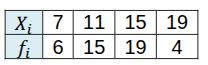
\includegraphics[scale=0.5]{ad1.png}
        \end{center} A mediana e a média aproximada valem, respectivamente:
        \begin{enumerate}[a]
            \item 14 e 13,76.
            \item \vermelho{15 e 12,91.}
            \item 14 e 14,80.
            \item 15 e 14,85.
            \item 16 e 14,90.

        \end{enumerate}        
    \end{frame}
\end{document}